% Template for Cogsci submission with R Markdown

% Stuff changed from original Markdown PLOS Template
\documentclass[10pt, letterpaper]{article}

\usepackage{cogsci}
\usepackage{pslatex}
\usepackage{float}
\usepackage{caption}

% amsmath package, useful for mathematical formulas
\usepackage{amsmath}

% amssymb package, useful for mathematical symbols
\usepackage{amssymb}

% hyperref package, useful for hyperlinks
\usepackage{hyperref}

% graphicx package, useful for including eps and pdf graphics
% include graphics with the command \includegraphics
\usepackage{graphicx}

% Sweave(-like)
\usepackage{fancyvrb}
\DefineVerbatimEnvironment{Sinput}{Verbatim}{fontshape=sl}
\DefineVerbatimEnvironment{Soutput}{Verbatim}{}
\DefineVerbatimEnvironment{Scode}{Verbatim}{fontshape=sl}
\newenvironment{Schunk}{}{}
\DefineVerbatimEnvironment{Code}{Verbatim}{}
\DefineVerbatimEnvironment{CodeInput}{Verbatim}{fontshape=sl}
\DefineVerbatimEnvironment{CodeOutput}{Verbatim}{}
\newenvironment{CodeChunk}{}{}

% cite package, to clean up citations in the main text. Do not remove.
\usepackage{apacite}

% KM added 1/4/18 to allow control of blind submission


\usepackage{color}

% Use doublespacing - comment out for single spacing
%\usepackage{setspace}
%\doublespacing


% % Text layout
% \topmargin 0.0cm
% \oddsidemargin 0.5cm
% \evensidemargin 0.5cm
% \textwidth 16cm
% \textheight 21cm

\title{Preschool children's understanding of polite requests}


\author{{\large \bf } \\ \texttt{} \\  \\}

\begin{document}

\maketitle

\begin{abstract}
As adults, we use polite speech on a daily basis. What do children
understand about polite speech? Looking at children's polite speech
comprehension can help examine children's pragmatic understanding more
generally, and can be informative for caregivers who want to teach
children what it means to be polite. Even though children start to
produce polite speech from early on, there is little known about whether
they understand intentions behind polite language. Here we show that by
3 years, English-speaking preschool children understand that it is more
polite and nicer (and less rude and mean) to use politeness markers such
as ``please'' when making requests, and by 4 years, they understand that
the use of these politeness markers indicates that the speaker is more
socially likeable and is more likely to gain compliance from their
conversational partners. This work can help lay the foundation for
future work on children's understanding of polite speech and pragmatic
development more generally.

\textbf{Keywords:}
Politeness, pragmatic development, online experiment
\end{abstract}

\section{Introduction}\label{introduction}

We use and hear polite speech on a daily basis: polite utterances range
from simple words of apology (``sorry'') or gratitude (``thanks'') to
compliments (``I love your dress!'') and requests (``Can you please open
the window?''). Yet polite utterances are seemingly inefficient and even
misinformative: speakers say ``Can you please \ldots{}'' when it should
suffice to say, ``Open the window.'' These facts are a mystery for
frameworks which describe communication in terms of efficient
information transfer (e.g., Buhler, 1934; Goodman \& Stuhlmuller, 2013;
Shannon, 1948): If language is a tool for transferring information,
speakers should be as efficient as possible in their communication to
prioritize informativity. Nonetheless, everyday politeness is ubiquitous
in everyday language use, and adults tend to use strategies to be polite
even while arguing (Holtgraves, 1997).

So why do people speak politely? Linguistic theories assume that
people's utterance choices are motivated by social concerns, framed as
either maxims (Leech, 1983), social norms (Ide, 1989), or listener's
and/or speaker's public identity (\emph{face}; Brown \& Levinson, 1987).
For example, Brown \& Levinson (1987)'s theory predicts that if a
speaker's intended meaning contains a threat to the listener's face or
self-image, the speaker's utterance will be less direct and less
informative. For example, if a speaker considered that saying ``Open the
window'' will give the impression that she is in a position to give
orders to the listener, she could instead say ``Can you please open the
window?'', using a more indirect form of request to give the other
person a sense of autonomy or freedom from imposition (Clark \& Schunk,
1980). Thus, while it may hinder the goal of efficient information
transfer, using polite speech can help the speaker save the listener's
face while simultaneously communicating her own positive social goals
(Yoon, Tessler, Goodman, \& Frank, 2017).

Do children speak politely, and if so, what do they understand about
polite speech? Previous research shows that children begin producing
polite speech early on; They produce ``please'' at 2.5 years (Read \&
Cherry, 1978), and request forms increase in their variety and frequency
with age (Bates, 1976; Bates \& Silvern, 1977; Bock \& Hornsby, 1981;
Ervin-Tripp, 1982; Nippold, Leonard, \& Anastopoulos, 1982). Young
children learn to produce different forms of requests depending on
context: For example, by three years children are able to vary their
utterances based on whether they are instructed to ``tell'' versus
``ask'' an addressee to given them a puzzle piece (Bock \& Hornsby,
1981). And even at two years, children are able to modify their requests
to make them more polite (``ask in the nicest way possible''; Bates \&
Silvern, 1977). Hence, children's production of polite speech seems to
parallel adult speakers' desires to produce utterances with appropriate
levels of face-saving.

While children appear to produce polite speech from an early age, less
is known about whether they \emph{understand} polite speech. Examining
children's comprehension of polite speech is important for a number of
reasons. First, children's polite speech understanding can reveal their
inferential abilities underlying more general pragmatic understanding:
going beyond what was literally said to infer what was intended. For
example, children need to understand that, in saying ``can you open the
window?'' the speaker does not literally question the listener's ability
to open the window but rather wants to make a polite request. Thus,
understanding what children comprehend about polite speech can help see
how children are able to infer speaker's intentions behind utterances.

Second, understanding polite speech can have practical implications for
education, as caregivers often care about teaching their children to be
more polite. Indeed, from very early on, parents teach children to
follow normative rituals to say ``please'', ``thank you'', ``hello'' and
``good-bye'' (Gleason, Perlmann, \& Greif, 1984). It can be enlightening
to know whether and when children understand positive implications of
following these norms.

Third, examining children's \emph{comprehension} of polite speech as
compared to their \emph{production} is meaningful, in that children's
comprehension can reveal more abstract representations and inferences
about language than their productivity (e.g., Fisher, 2002): Children's
ability to say ``please'' early on does not necessarily indicate that
they understand saying ``please'' is more polite, nicer and socially
apt, as children may simply obey or imitate what their caregivers tell
them to say without understanding its meaning.

Research on children's comprehension of polite speech has received less
focus than research on their production of polite speech. Moreover, the
few studies that did examine children's understanding of polite speech
have been largely inconclusive. Though there was some initial evidence
to suggest that producing a request with ``please'' is judged to be
polite by three years of age (Bates, 1976; Bates \& Silvern, 1977), in a
later study, the judgment of ``please'' as being polite was only
replicated starting at five years of age, but not younger (Nippold et
al., 1982). These initial studies also lacked statistical tests to
assess each age group's performance, and did not systematically
manipulate cues other than linguistic markers (e.g., prosody or facial
expressions).

In addition to children's recognition of politeness markers, there are
also many open questions about their abilities to recognize the
intentions underlying polite speech. For example, do children know that
the word ``polite'' should be associated with politeness rules people
abide by (e.g., saying ``please'')? Relatedly, do children recognize
polite speech as being positively valenced, such that they think it is
better and nicer to say polite things? Do children understand the social
implications of speaking politely? For example, polite people may be
more likely to get their wishes granted (``I will pour him more water
because he was nice'') and may be better social play partners compared
to those who are impolite. Finally, what cues to politeness do children
recognize? Do they recognize linguistic politeness markers such as
``please,'' or ``can you,'' or both? Or do they rely on prosodic cues
that make utterances sound more respectful, or on facial expressions
that make a person look kind?

In this current work, we sought to answer these questions, and test what
2- to 4-year-old children understand about requests using politeness
markers. Across three experiments, we presented stories about speakers
who decided to speak politely (e.g., ``Please pour me more water'') or
impolitely (``Pour me more water'') and asked child participants to make
judgments between the two speakers. We examined in each experiment
whether: (1) children are able to reason about speakers using polite
speech as being relatively more ``polite'' and ``nice'' and less
``rude'' or ``mean'' than speakers not using polite speech; (2) they can
reason about social implications of using polite speech (e.g.,
politeness as a sign of a nice play partner, or greater likelihood of
compliance from the addressee); and (3) they show improvement with age
for these lines of reasoning. We also examined whether children need
additional cues to politeness such as facial expressions (Expt 1) or
prosodic cues (Expt 2), or they can make use of linguistic politeness
markers alone (Expt 3) to make appropriate inferences about speakers.

\section{Experiment 1}\label{experiment-1}

In Experiment 1, we tested whether 3- to 4-year-old children were able
to understand the implications of using simple politeness markers, based
on linguistic cues of interest (whether the speaker says ``please,''
``can you'') and other cues (facial expressions and prosodic cues) that
make polite speech more salient and naturalistic.

\subsection{Methods}\label{methods}

\subsubsection{Participants}\label{participants}

3-year-old (\(n=\) 20; 12 F, \(M_{age}\) = 3.61 years, \(SD_{age}\) =
0.22) and 4-year-old children (\(n=\) 18; 6 F, \(M_{age}\) = 4.38 years,
\(SD_{age}\) = 0.25) were recruited from a local preschool. An
additional 3 children were tested but excluded due to failure on the
practice questions (\(n=\) 2) or completion of fewer than half of the
test trials (\(n=\) 1).

\subsubsection{Stimuli and design}\label{stimuli-and-design}

We designed a picture book with twelve stories in which a protagonist is
approached by two speakers, one of whom makes a request by producing an
utterance with a politeness marker (e.g., ``Please pour me more
water''), and the other produces an utterance without (``Pour me more
water''). There were three types of politeness marker that could be
used: ``please'' (as in ``Please pour me more water''), ``can you''
(``Can you pour me more water''), and ``can you please'' (``Can you
please pour me more water'').

We designed six question types to ask participants following the
presentation of the stories: four \emph{speaker attribute} questions
(\emph{polite}: ``Which one was more polite?''; \emph{rude}: ``Which one
was more rude?''; \emph{nice}: ``Which one was nicer?''; \emph{mean}:
``Which one was meaner?'') and two \emph{social implication} questions
(\emph{play partner}: ``Which one would you rather play with?'';
\emph{compliance}: ``Which one will {[}get what they want{]}?''). Each
participant would be asked one of the four speaker attribute questions,
followed by one of the two social implication questions.

In Experiment 1, all utterances were produced live by the experimeter,
with appropriate proodic cues and facial expressions for each request:
Utterances with politeness markers were produced by kind voice and
facial expression, whereas utterances lacking politeness marker were
produced with angry voice and facial cues.

\subsubsection{Procedure}\label{procedure}

The experimenter presented to the child a storybook with a total of
thirteen stories about different characters. In the \emph{practice}
phase, the child heard a story with one clearly mean character
(\emph{Drew kicked Carol}) and one clearly nice character (\emph{Graham
gave Carol a gift}). After a reminder of what each character did, the
experimenter asked the participant: \emph{Which one was being meaner?}
and \emph{Which one was being nicer?} If the child answered the question
wrong the first time, the experimenter read the story one more time,
saying, ``Let's think about the story one more time.'' Only children who
correctly answered both questions in the first or second attempt were
included in the analyses.

In the \emph{test} phase, the child heard twelve stories, in each of
which they saw one speaker who decided to speak politely (\emph{Jean
wanted more water in her cup. Jean said to Fred, ``Please pour me more
water''}) and another speaker who spoke impolitely (\emph{Suzy also
wanted more water in her cup. Suzy said to Fred, ``Pour me more
water.''}). After a reminder about what each speaker said, the child was
asked a total of two questions. For the first question, the experimenter
asked one out of four possible questions for speaker attribute: ``Which
one was being more polite {[}more rude/nicer/meaner{]}?'' For the
second, social implication question, the experimenter either asked about
play partner (\emph{Which one would you rather play with?}) or
likelihood of compliance (e.g., \emph{Which one will Fred give water
to?}). The order of story types and question types was counterbalanced.

\subsection{Results and Discussion}\label{results-and-discussion}

\begin{CodeChunk}
\begin{figure*}[h]

{\centering 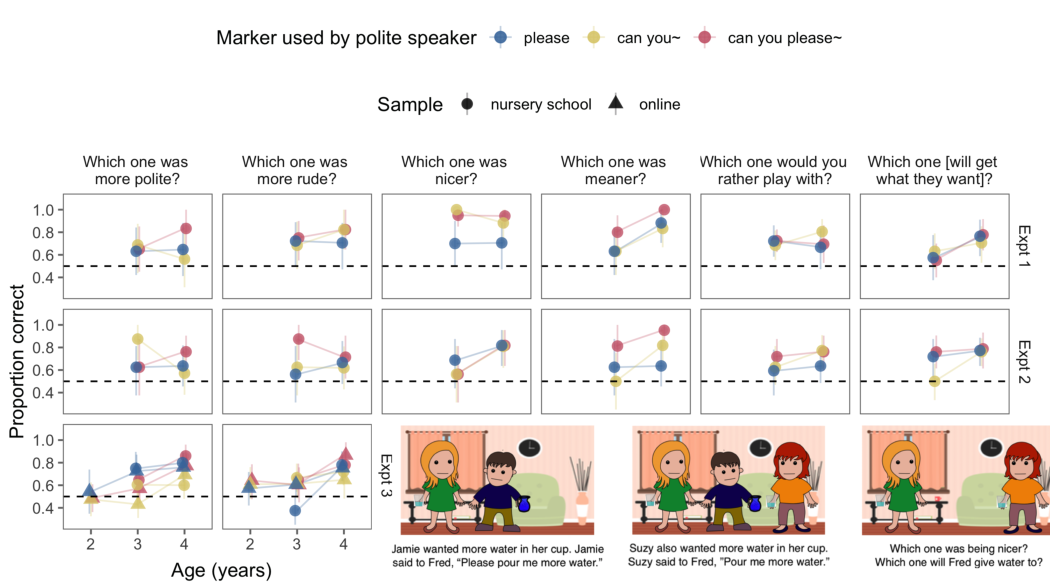
\includegraphics{figs/fig_results_placement-1} 

}

\caption[Bottom right]{Bottom right: Story example. Top, left: Results. Proportion of correct responses to questions comparing between a speaker who used a politeness marker (where blue indicates "please", yellow "can you", and red "can you please") versus a speaker who did not. Data are binned into one-year age groups. Each row represents data from a different Experiment. Columns represent different questions asked. Dashed line represents chance level at 50\% (i.e., if participant were guessing at random).}\label{fig:fig_results_placement}
\end{figure*}
\end{CodeChunk}

We looked at the proportion of correct responses to various questions
comparing speakers who used a politeness marker and spoke kindly, and
speakers who did not use a politeness marker and spoke meanly
(Figure~\ref{fig:fig_results_placement}, first row). A mixed-effects
logistic regression predicting accuracy based on age, question type and
politeness marker type\footnote{for Experiments 1 and 2, we use this
  model structure with a maximal random effect structure that converges:
  \texttt{accuracy\ \textasciitilde{}\ age\ x\ question\ type\ x\ politeness\ marker\ type\ +\ (1\ \textbar{}\ item)},
  where age is continuous, centered and scaled. All categorical
  variables were deviation coded, with specified contrasts of interest
  for the question type. Significance was calculated using the standard
  normal approximation to the \(t\) distribution (Barr, Levy, Scheepers,
  \& Tily, 2013).} showed there was an improvement with age (\(\beta\) =
0.2, \(p =\) 0.026). The regression model also revealed that children
seemed to find some question types easier than others: Responses to
\emph{nice} and \emph{mean} questions were more accurate than to
\emph{polite} and \emph{rude} questions (\(\beta\) = 0.8, \(p =\)
0.002), whereas social implication questions (\emph{play partner} and
\emph{compliance}) were overall more difficult compared to speaker
attribute questions (\emph{polite}, \emph{rude}, \emph{nice}, and
\emph{mean}; \(\beta\) = -0.33, \(p =\) 0.006).

Looking more closely at responses for each of the question types,
children from both age groups tended to accurately answer the
\emph{polite}, \emph{nice}, \emph{mean}, \emph{rude}, and \emph{play
partner} questions overall (3-year-olds' mean accuracy range: 0.58 -
0.88; 4-year-olds' mean accuracy range: 0.68 - 0.9), indicating
correctly that the speaker who used a politeness marker was more polite
and nicer, and less mean and rude, and was likely a better play partner.
For the \emph{compliance} question, 4-year-olds overall answered
correctly that the speaker who used politeness marker will likely get
what they want from the listener (\(M_{4y}\) = 0.75, \(p\) \textless{}
.01), but 3-year-olds did not perform above chance (\(M_{3y}\) = 0.58).
As for the different politeness marker types, both age groups overall
tended to give correct answers based on all three markers, but
especially ``can you please'' (3-year-olds: \(M_{please}\) = 0.66,
\(M_{can you}\) = 0.72, \(M_{can you please}\) = 0.74; 4-year-olds:
\(M_{please}\) = 0.73, \(M_{can you}\) = 0.77, \(M_{can you please}\) =
0.84).

In sum, in this first experiment, we saw preliminary evidence that
children pay attention to some cues to politeness and are able to use
these cues to infer whether speakers are relatively polite, rude, nice
or mean, and whether speakers are good play partners and are likely to
get what they wanted from their addressees. 4-year-olds answered
questions accurately more often compared to 3-year-olds, especially for
the question about addressee's compliance with the speaker's request. In
general, however, both age groups tended to be accurate when all the
possible cues were used to signal that one speaker was polite (used
``can you please'', spoke with a kind tone and face) and the other
speaker wasn't (did not use a politeness marker, spoke with an angry
tone and face).

There were a number of remaining issues from Experiment 1. Children may
not have used the linguistic politeness markers (e.g., ``please'') per
se, and rather prosodic and facial cues that accompany these markers.
That is, children may have relied on the speaker's kind voice and face
rather than their use of ``please'' to evaluate their niceness or
likeability as a play partner. Similarly, greater accuracy for some
questions over others (e.g., \emph{nice} \textgreater{} \emph{polite})
may have been due to greater association between some of the words and
prosodic and facial cues (e.g., a kind face may be seen to signal
niceness more than politeness), not due to greater understanding for
those words or concepts. Another concern is that the experimenter was
aware of the manipulations (i.e., they knew which speaker was supposed
to be ``polite'') and thus could have affected the presentation of these
speakers in ways that are not consistent across all participants. In our
next two experiments, we sought to remove these potential confounds.

\section{Experiment 2}\label{experiment-2}

In Experiment 1, we saw initial evidence that children can use some
combinations of linguistic, prosodic, and facial cues to politeness. In
Experiment 2, we examined whether children can make similar judgments
using linguistic and prosodic cues only, without facial expressions. For
this, we conducted a preregistered experiment where we used pre-recorded
voiceovers to present speaker utterances, so that (1) we could look at
children's judgments based on linguistic markers and prosodic cues only,
and (2) we could remove the role of the experimenter in presentation of
these utterances.

\subsection{Methods}\label{methods-1}

\subsubsection{Participants}\label{participants-1}

3-year-old (\(n=\) 16; 8 F, \(M_{age}\) = 3.56 years, \(SD_{age}\) =
0.29) and 4-year-old children (\(n=\) 22; 13 F, \(M_{age}\) = 4.5 years,
\(SD_{age}\) = 0.32) were recruited from a local preschool. An
additional 5 children were tested but excluded due to failure on the
practice questions.

\subsubsection{Stimuli and design}\label{stimuli-and-design-1}

The design was identical to Experiment 1. Stimuli were the same as
Experiment 1 except two changes: (1) Instead of a picture book, we
presented the stories on a tablet; (2) the speakers' utterances were now
presented as recorded voiceovers. The voiceovers were recorded by native
English speakers, and contained prosodic cues that matched the
presence/absence of a politeness marker (e.g., ``Please pour me more
water'' was recorded with a kind voice and ``pour me more water'' with
an angry voice).

\subsubsection{Procedure}\label{procedure-1}

The procedure was identical to Experiment 1, except for the following
change: The participants now had to tap on a speaker on tablet in order
either to hear them speak, or to choose an answer to the questions
asked.

\subsection{Results and Discussion}\label{results-and-discussion-1}

Overall we saw similar patterns of results in Experiment 2
(Figure~\ref{fig:fig_results_placement}, second row) compared to Exp. 1.
A mixed-effects logistic regression predicting accuracy based on age,
question type and politeness marker type showed that accuracy improved
with age (\(\beta\) = 0.25, \(p =\) 0.002), and children made accurate
judgments more often when the politeness marker was ``can you please''
than when the marker was ``please'' or ``can you'' (\(\beta\) = 0.33,
\(p =\) 0.019). There was no main effect of question type, but there was
an interaction between age and question type such that performance for
\emph{nice} and \emph{mean} questions saw greater improvement with age
than for \emph{polite} and \emph{rude} questions (\(\beta\) = 0.57,
\(p =\) 0.011).

For children's responses to different question types, 3-year-olds'
accuracy did not differ from chance level for \emph{nice}, \emph{mean},
and \emph{play partner} questions, but their means numerically exceeded
50\% for all question types, and 4-year-olds accurately answered
questions of all types (3-year-olds' mean accuracy range: 0.6 - 0.88;
4-year-olds' mean accuracy range: 0.66 - 0.9). For politeness marker
types, 3-year-olds' performance did not differ from chance for
``please'' and ``can you'', but both age groups tended to answer
questions about different politeness markers accurately overall
(3-year-olds: \(M_{please}\) = 0.63, \(M_{can you}\) = 0.61,
\(M_{can you please}\) = 0.72; 4-year-olds: \(M_{please}\) = 0.7,
\(M_{can you}\) = 0.72, \(M_{can you please}\) = 0.8).

In sum, across Experiments 1 and 2, we saw that children tend to make
accurate judgments about speakers given their use of politeness markers,
especially ``can you please,'' together with prosodic cues, and children
get better with age in their use of politeness cues to respond to
questions about speaker attributes and social implications.

\section{Experiment 3}\label{experiment-3}

We conducted a third, pre-registered experiment to see whether children
are able to evaluate speakers based on linguistic markers only, without
any other supporting cues such as prosodic cues or facial expressions.

\subsection{Methods}\label{methods-2}

\subsubsection{Participants}\label{participants-2}

We recruited two samples of participants: one from the same local
nursery school as Experiments 1 and 2, and the other from Lookit
(\url{https://lookit.mit.edu/}), an online platform for child research
participation, in which parents and their children can participate
together. The nursery school sample consisted of 3-year-old (\(n=\) 24;
11 F, \(M_{age}\) = 3.65 years, \(SD_{age}\) = 0.26) and 4-year-old
children (\(n=\) 25; 13 F, \(M_{age}\) = 4.48 years, \(SD_{age}\) =
0.28). An additional 3 children were tested but excluded due to failure
on the practice questions. The online sample consisted of 2-year-old
(\(n=\) 23; 12 F, \(M_{age}\) = 2.48 years, \(SD_{age}\) = 0.29),
3-year-old (\(n=\) 31; 15 F, \(M_{age}\) = 3.59 years, \(SD_{age}\) =
0.27) and 4-year-old children (\(n=\) 27; 12 F, \(M_{age}\) = 4.46
years, \(SD_{age}\) = 0.29). An additional 32 children were tested but
excluded due to failure on the practice questions (\(n=\) 19) or
completion of fewer than half of the test trials (\(n=\) 13).

\subsubsection{Stimuli}\label{stimuli}

For the nursery school sample, stimuli were identical to Experiment 2
except that the voiceovers for all utterances had the same prosody: All
utterances ended with a rising intonation. For the online sample,
stimuli were identical to what the nursery school participants saw
except that the story narrations (other than speaker utterances) were
also pre-recorded such that parents did not need to read the stories
aloud to their children.

\subsubsection{Procedure}\label{procedure-2}

For the nursery school sample, the procedure was identical to Experiment
2. For the online sample, the procedure was similar except that parents
and children participated together at home and there was no experimenter
present. Parents accessed the webpage for the study and gave their
consent for participation, and then read instructions to proceed through
the different stories, which specifically asked the parents to not tell
their children correct answers for the questions.

\subsection{Results and Discussion}\label{results-and-discussion-2}

\subsubsection{Experiment 3}\label{experiment-3-1}

For Experiment 3, we were able to look at how children answered the
\emph{polite} and \emph{rude} questions given the same three politeness
marker types as in Experiments 1 and 2, with three age groups including
2-year-olds. (Fig. ~\ref{fig:fig_results_placement}, third row).

A mixed-effects logistic regression controlling for the effect of
sample\footnote{Model structure:
  \texttt{accuracy\ \textasciitilde{}\ sample\ +\ age\ x\ question\ type\ x\ politeness\ marker\ type\ +\ (1\ \textbar{}\ item)}}
showed improvement with age (\(\beta\) = 0.19, \(p =\) 0.033) as well as
better performance for ``can you please'' than ``please'' and ``can
you'' together (\(\beta\) = 0.42, \(p =\) 0.002), consistent with
Experiment 2 results. Performance for ``please'' was also better than
for ``can you please'' and ``please'' together (\(\beta\) = 0.3, \(p =\)
0.027), which may be surprising given that we previously did not see the
same effect in Experiments 1 and 2. One possible explanation is that
controlling for prosodic cues in Experiment 3 actually made it
\emph{easier} to use ``please'' as a politeness cue. Because we had
stripped all the other variations, it may have made the contrast between
the presence and absence of the marker ``please'' \emph{more} salient.

Additionally, children were better with the \emph{polite} questions than
\emph{rude} overall (\(\beta\) = -0.19, \(p =\) 0.04), but especially
given ``please'' (\(\beta\) = 0.42, \(p =\) 0.002). Finally, children
showed a greater improvement with age for ``can you please'' compared to
``please'' and ``can you'' together (\(\beta\) = 0.38, \(p =\) 0.004).

\subsubsection{All experiments}\label{all-experiments}

Did children perform better given facial and/or prosodic cues, or were
linguistic politeness markers sufficient? To see any potential effect of
experiment on children's performance, we conducted an exploratory
mixed-effects logistic regression on all three experiments
together\footnote{Model structure:
  \texttt{accuracy\ \textasciitilde{}\ sample\ +\ experiment\ +\ age\ x\ question\ type\ x\ politeness\ marker\ type\ +\ (1\ \textbar{}\ item)}}.
The regression model showed no significant main effect of experiment,
suggesting that children did not perform more poorly when facial and
prosodic cues were removed, and they were able to make accurate
judgments based on linguistic cues alone. The model also showed that
children improved with increasing age (\(\beta\) = 0.33, \(p\)
\textless{} .001) and that children were more accurate with ``can you
please'' than ``please'' and ``can you'' (\(\beta\) = 0.25, \(p =\)
0.011), confirming results from each individual experiment.
Additionally, the model showed that children became better at judging
the politeness marker ``can you please'' with age (\(\beta\) = 0.73,
\(p =\) 0.005), and that children answered \emph{polite} questions
better than \emph{rude} questions about the marker ``please'' (\(\beta\)
= 0.26, \(p =\) 0.006)

\section{General Discussion}\label{general-discussion}

What do young children understand about polite speech? In three
experiments, we looked at how 2- to 4-year-old children reason about
making requests with or without simple politeness markers such as
``please'', ``can you'' and ``can you please.'' By 3 years, children pay
attention to the use of politeness markers to accurately judge whether
that speaker is relatively more polite, rude, nicer or meaner compared
to another speaker. By 4 years, children reliably infer that a speaker
who uses a politeness marker is a better play partner and more likely to
get what they want. Across all three experiments, we saw a clear
developmental trend such that children improved in their reasoning about
polite speech with increasing age. We observed no large experiment
effects as we eliminated facial and prosodic cues; instead, all these
inferences appeared to be supported by linguistic markers alone.

Even though children have been shown to produce polite speech such as
``please,'' evidence has been sparse and inconclusive for whether young
children below 5 years comprehend speaker attributes and intentions
based on polite speech. Here, we found that children are sensitive to
the use of politeness markers in speech, and are able to use these
markers to infer the speaker's attributes (e.g., niceness) by 3 years,
and consequent social implications by 4 years. These ages are closer to
the age of first reliable production of polite speech than have been
suggested by earlier work.

Children in the US are often explicitly taught and prompted to use
politeness markers such as ``please'' in their requests from early on
(e.g., ``What's the magic word?''; Gleason et al., 1984), thus they may
quickly learn to use these markers as a rule in order to get what they
want. They also might hear other remarks that pair politeness markers
with positive words (e.g., ``You should be \emph{nice} and say
\emph{please}''), which may help them learn the association between
polite speech and positive attributes. Gradually, children may recognize
more subtle social processes that are related to polite speech
production: Adults may praise and reward children who spoke politely,
and children themselves may like peers who ask for permission to play
with their toys rather than take the toys away without asking. Future
work with corpus data analysis looking at these interactions between
children and others may reveal important conversational patterns that
help children acquire social meanings of polite speech.

There are limitations to the current work that present other
opportunities for future research. Because this work looked only at the
behaviors of English-speaking children with a relatively high
socioeconomic status in the US, it is an open question how children with
different language and cultural background may develop understanding of
polite speech. Cross-cultural investigation of what markers are present
in other languages, cultures and backgrounds, as well as how those
markers are acquired, will be informative.

Also, we did not manipulate the social status of speakers or addressees.
Though not explicitly stated, the visual depiction and narration used
for the current work suggested that speakers were communicating with
their peers only. However, one key prediction from politeness theory is
that speakers will adjust their utterances based on the status of the
addressees (Brown \& Levinson, 1987). Indeed children adjust own their
speech based on the listener status and age: Even at two years, children
use a polite form of request (``Can I have\ldots{}'') to an adult but an
imperative form (``Give me\ldots{}'') to a peer (Shatz \& Gelman, 1973).
Thus, future work should examine how children use cues to politeness to
judge speaker intentions in different contexts, including varied status
differences between speakers and listeners.

In sum, the current work showed that young children understand
implications of using simple politeness markers in requests. A broader
understanding of the emergence of politeness may offer insights into how
children become proficient users of language across the wide range of
social situations that they encounter.

\vspace{1em}
\fbox{\parbox[b][][c]{7.3cm}{\centering All experiments, data, and analysis code are available in the public repository for the project: (link will be available upon acceptance)}}
\vspace{1em} \noindent

\section{References}\label{references}

\setlength{\parindent}{-0.1in} \setlength{\leftskip}{0.125in} \noindent

\hypertarget{refs}{}
\hypertarget{ref-barr2013}{}
Barr, D. J., Levy, R., Scheepers, C., \& Tily, H. J. (2013). Random
effects structure for confirmatory hypothesis testing: Keep it maximal.
\emph{Journal of Memory and Language}, \emph{68}(3), 255--278.

\hypertarget{ref-bates1976}{}
Bates, E. (1976). Acquisition of polite forms: Experimental evidence.
\emph{Language and Context: The Acquisition of Pragmatics}, 295--326.

\hypertarget{ref-bates1977}{}
Bates, E., \& Silvern, L. (1977). Social adjustment and politeness in
preschoolers. \emph{Journal of Communication}, \emph{27}(2), 104--111.

\hypertarget{ref-bock1981}{}
Bock, J. K., \& Hornsby, M. E. (1981). The development of directives:
How children ask and tell. \emph{Journal of Child Language},
\emph{8}(01), 151--163.

\hypertarget{ref-brown1987}{}
Brown, P., \& Levinson, S. C. (1987). \emph{Politeness: Some universals
in language usage} (Vol. 4). Cambridge university press.

\hypertarget{ref-buhler1934}{}
Buhler, K. (1934). \emph{Sprachtheorie}. Oxford, England: Fischer.

\hypertarget{ref-clark1980}{}
Clark, H. H., \& Schunk, D. H. (1980). Polite responses to polite
requests. \emph{Cognition}, \emph{8}(2), 111--143.

\hypertarget{ref-ervin1982}{}
Ervin-Tripp, S. M. (1982). Ask and it shall be given unto you:
Children's requests. \emph{Georgetown University Roundtable on Languages
and Linguistics. Contemporary Perceptions of Language: Interdisciplinary
Dimensions}, 235--245.

\hypertarget{ref-fisher2002}{}
Fisher, C. (2002). The role of abstract syntactic knowledge in language
acquisition: A reply to tomasello (2000). \emph{Cognition},
\emph{82}(3), 259--278.

\hypertarget{ref-gleason1984}{}
Gleason, J. B., Perlmann, R. Y., \& Greif, E. B. (1984). What's the
magic word: Learning language through politeness routines?
\emph{Discourse Processes}, \emph{7}(4), 493--502.

\hypertarget{ref-goodman2013}{}
Goodman, N. D., \& Stuhlmuller, A. (2013). Knowledge and implicature:
Modeling language understanding as social cognition. \emph{Topics in
Cognitive Science}, \emph{5}(1), 173--184.

\hypertarget{ref-holtgraves1997}{}
Holtgraves, T. (1997). YES, but... positive politeness in conversation
arguments. \emph{Journal of Language and Social Psychology},
\emph{16}(2), 222--239.

\hypertarget{ref-ide1989}{}
Ide, S. (1989). Formal forms and discernment: Two neglected aspects of
universals of linguistic politeness. \emph{Multilingua-Journal of
Cross-Cultural and Interlanguage Communication}, \emph{8}(2-3),
223--248.

\hypertarget{ref-leech1983}{}
Leech, G. (1983). \emph{Principles of pragmatics}. London, New York:
Longman Group Ltd.

\hypertarget{ref-nippold1982}{}
Nippold, M. A., Leonard, L. B., \& Anastopoulos, A. (1982). Development
in the use and understanding of polite forms in children. \emph{Journal
of Speech, Language, and Hearing Research}, \emph{25}(2), 193--202.

\hypertarget{ref-read1978}{}
Read, B. K., \& Cherry, L. J. (1978). Preschool children's production of
directive forms. \emph{Discourse Processes}, \emph{1}(3), 233--245.

\hypertarget{ref-shannon1948}{}
Shannon, C. E. (1948). A mathematical theory of communication.
\emph{Bell Syst. Tech. J.}, \emph{27}, 623--656.

\hypertarget{ref-shatz1973}{}
Shatz, M., \& Gelman, R. (1973). The development of communication
skills: Modifications in the speech of young children as a function of
listener. \emph{Monographs of the Society for Research in Child
Development}, 1--38.

\hypertarget{ref-yoon2017}{}
Yoon, E. J., Tessler, M. H., Goodman, N. D., \& Frank, M. C. (2017). ``I
won't lie, it wasn't amazing": Modeling polite indirect speech. In
\emph{Proceedings of the thirty-ninth annual conference of the Cognitive
Science Society}.

\bibliographystyle{apacite}


\end{document}
